% ------------------------------------------------------------------------
% ------------------------------------------------------------------------
% abnTeX2: Modelo de Trabalho Academico (tese de doutorado, dissertacao de
% mestrado e trabalhos monograficos em geral) em conformidade com
% ABNT NBR 14724:2011: Informacao e documentacao - Trabalhos academicos -
% Apresentacao
% ------------------------------------------------------------------------
% ------------------------------------------------------------------------

\documentclass[
	% -- opções da classe memoir --
	12pt,				% tamanho da fonte
	openright,			% capítulos começam em pág ímpar (insere página vazia caso preciso)
	twoside,			% para impressão em recto e verso. Oposto a oneside
	a4paper,			% tamanho do papel.
	% -- opções da classe abntex2 --
	%chapter=TITLE,		% títulos de capítulos convertidos em letras maiúsculas
	%section=TITLE,		% títulos de seções convertidos em letras maiúsculas
	%subsection=TITLE,	% títulos de subseções convertidos em letras maiúsculas
	%subsubsection=TITLE,% títulos de subsubseções convertidos em letras maiúsculas
	% -- opções do pacote babel --
	english,			% idioma adicional para hifenização
	brazil,				% o último idioma é o principal do documento
	svgnames
	]{abntex2}\usepackage[]{graphicx}\usepackage[]{color}
% maxwidth is the original width if it is less than linewidth
% otherwise use linewidth (to make sure the graphics do not exceed the margin)
\makeatletter
\def\maxwidth{ %
  \ifdim\Gin@nat@width>\linewidth
    \linewidth
  \else
    \Gin@nat@width
  \fi
}
\makeatother

\definecolor{fgcolor}{rgb}{0.345, 0.345, 0.345}
\newcommand{\hlnum}[1]{\textcolor[rgb]{0.686,0.059,0.569}{#1}}%
\newcommand{\hlstr}[1]{\textcolor[rgb]{0.192,0.494,0.8}{#1}}%
\newcommand{\hlcom}[1]{\textcolor[rgb]{0.678,0.584,0.686}{\textit{#1}}}%
\newcommand{\hlopt}[1]{\textcolor[rgb]{0,0,0}{#1}}%
\newcommand{\hlstd}[1]{\textcolor[rgb]{0.345,0.345,0.345}{#1}}%
\newcommand{\hlkwa}[1]{\textcolor[rgb]{0.161,0.373,0.58}{\textbf{#1}}}%
\newcommand{\hlkwb}[1]{\textcolor[rgb]{0.69,0.353,0.396}{#1}}%
\newcommand{\hlkwc}[1]{\textcolor[rgb]{0.333,0.667,0.333}{#1}}%
\newcommand{\hlkwd}[1]{\textcolor[rgb]{0.737,0.353,0.396}{\textbf{#1}}}%
\let\hlipl\hlkwb

\usepackage{framed}
\makeatletter
\newenvironment{kframe}{%
 \def\at@end@of@kframe{}%
 \ifinner\ifhmode%
  \def\at@end@of@kframe{\end{minipage}}%
  \begin{minipage}{\columnwidth}%
 \fi\fi%
 \def\FrameCommand##1{\hskip\@totalleftmargin \hskip-\fboxsep
 \colorbox{shadecolor}{##1}\hskip-\fboxsep
     % There is no \\@totalrightmargin, so:
     \hskip-\linewidth \hskip-\@totalleftmargin \hskip\columnwidth}%
 \MakeFramed {\advance\hsize-\width
   \@totalleftmargin\z@ \linewidth\hsize
   \@setminipage}}%
 {\par\unskip\endMakeFramed%
 \at@end@of@kframe}
\makeatother

\definecolor{shadecolor}{rgb}{.97, .97, .97}
\definecolor{messagecolor}{rgb}{0, 0, 0}
\definecolor{warningcolor}{rgb}{1, 0, 1}
\definecolor{errorcolor}{rgb}{1, 0, 0}
\newenvironment{knitrout}{}{} % an empty environment to be redefined in TeX

\usepackage{alltt}

% ---
% Novo list of (listings) para QUADROS
% ---

%\newcommand{\quadroname}{Quadro}
%\newcommand{\listofquadrosname}{Lista de quadros}

%\newfloat[chapter]{quadro}{loq}{\quadroname}
%\newlistof{listofquadros}{loq}{\listofquadrosname}
%\newlistentry{quadro}{loq}{0}

% configurações para atender às regras da ABNT
%\counterwithout{quadro}{chapter}
%\renewcommand{\cftquadroname}{\quadroname\space}
%\renewcommand*{\cftquadroaftersnum}{\hfill--\hfill}

% ---
% PACOTES
% ---
\usepackage{lscape}
% ---
% Pacotes fundamentais
% ---
\usepackage{lmodern}			% Usa a fonte Latin Modern
\usepackage[T1]{fontenc}		% Selecao de codigos de fonte.
\usepackage[utf8]{inputenc}		% Codificacao do documento (conversão automática dos acentos)
\usepackage{indentfirst}		% Indenta o primeiro parágrafo de cada seção.
\usepackage{color}			% Controle das cores
\usepackage{graphicx}			% Inclusão de gráficos
\usepackage{microtype} 			% para melhorias de justificação
\usepackage{setspace}
\usepackage{wrapfig}

% ---
% Para titulo em destaque sem sequencia de numeração
% ---
\newcommand{\datatitle}[1]{
  \normalsize \textsc{#1}
}

% ---
% Funções matematicas
% ---
\usepackage{amsmath,amssymb,amstext}
\usepackage{mathtools}                  % Funcionalidades (como \dcases)
\usepackage{dsfont}    %% Para \mathds{1} Indicadora
\usepackage{bm}

\DeclareMathOperator{\Ell}{\mathcal{L}}
\DeclareMathOperator{\R}{\mathbb{R}}
\DeclareMathOperator{\ind}{\mathds{1}}

\DeclareRobustCommand{\rchi}{{\mathpalette\irchi\relax}}
\newcommand{\irchi}[2]{\raisebox{\depth}{$#1\chi$}}

% ---
% Para tabelas
% ---
\usepackage{multirow}
\usepackage{array}
\usepackage{threeparttable}

% ---
% Pacotes e definições adcionais, para adequações especificas
% ---
\usepackage{tikz}
\usepackage{pdflscape}			% para ambiente landscape
\usepackage{pgfgantt}			% cronograma estilo gráfico de gantt
\usepackage{multicol}
\usetikzlibrary{backgrounds}
\usepackage{tasks}

% ---
% Fontes matemáticas
% ---
\usepackage{mathpazo}
\usepackage{inconsolata}
\usepackage{verbatim}

% ---
% Pacotes adicionais, usados apenas no âmbito do Modelo Canônico do abnteX2
% ---
\usepackage{lipsum}				% para geração de dummy text
% ---

% ---
% Pacotes de citações
% ---
\usepackage[brazilian,hyperpageref]{backref}% Paginas com as citações
\usepackage[alf, abnt-etal-list=0]{abntex2cite}				% Citações padrão ABNT

% ---
% CONFIGURAÇÕES DE PACOTES
% ---

% ---
% Configurações do pacote backref
% Usado sem a opção hyperpageref de backref
\renewcommand{\backrefpagesname}{Citado na(s) página(s):~}
% Texto padrão antes do número das páginas
\renewcommand{\backref}{}
% Define os textos da citação
\renewcommand*{\backrefalt}[4]{
  \ifcase #1 %
  Nenhuma citação no texto.%
  \or
  Citado na página #2.%
  \else
  Citado #1 vezes nas páginas #2.%
  \fi}%
% ---

% ---
% Informações de dados para CAPA e FOLHA DE ROSTO
% ---
\titulo{Aprendizado de máquina \\ Laboratório 2 - Impactos da base de aprendizagem para diferentes algoritmos de classificação}
\vspace{2cm}
\autor{Lineu Alberto Cavazani de Freitas}
\local{Curitiba}
\data{2021}
\instituicao{Universidade Federal do Paraná}

\preambulo{Relatório apresentado à disciplina
    Aprendizado de Máquina, ministrada pelo professor Luiz Eduardo Soares de Oliveira, no Programa de Pós Graduação em Informática da Universidade Federal do Paraná.}
% ---

% ---
% Configurações de aparência do PDF final

% informações do PDF
\makeatletter
\hypersetup{
  % pagebackref=true,
  pdftitle={\@title},
  pdfauthor={\@author},
  pdfsubject={\imprimirpreambulo},
  pdfcreator={LaTeX with abnTeX2},
  % pdfkeywords={abnt}{latex}{abntex}{abntex2}{projeto de pesquisa},
  colorlinks=true,	% false: boxed links; true: colored links
  linkcolor=blue,     % color of internal links
  citecolor=blue, % color of links to bibliography
  filecolor=magenta, % color of file links
  urlcolor=black,
  bookmarksdepth=4
}
\addto\captionsbrazil{
  \renewcommand{\bibname}{REFER\^ENCIAS}
}
\makeatother
% ---

% ---
% Espaçamentos entre linhas e parágrafos
% ---

% O tamanho do parágrafo é dado por:
\setlength{\parindent}{1.3cm}

% Controle do espaçamento entre um parágrafo e outro:
\setlength{\parskip}{0.2cm}  % tente também \onelineskip

% ---
% Highlight knitr code (pode-usar usar os varios highligths já definidos
% com thm = knit_theme$get("nuvola"); knit_theme$set(thm))
% ---

\renewcommand{\hlnum}[1]{\textcolor[rgb]{0.733,0,1}{#1}}%
\renewcommand{\hlstr}[1]{\textcolor[rgb]{0,0.533,0}{#1}}%
\renewcommand{\hlcom}[1]{\textcolor[rgb]{0,0,0}{#1}}%
\renewcommand{\hlopt}[1]{\textcolor[rgb]{0.412,0.412,0.412}{#1}}%
\renewcommand{\hlstd}[1]{\textcolor[rgb]{0.2,0.2,0.2}{{#1}}}%
\renewcommand{\hlkwa}[1]{\textcolor[rgb]{0.2,0.2,0.2}{{#1}}}%
\renewcommand{\hlkwb}[1]{\textcolor[rgb]{0.4,0,0}{\textbf{#1}}}%
\renewcommand{\hlkwc}[1]{\textcolor[rgb]{0.13,0.29,0.53}{#1}}%
\renewcommand{\hlkwd}[1]{\textcolor[rgb]{0.13,0.29,0.53}{\textbf{#1}}}%

% ---
% compila o indice
% ---
\makeindex
% ---

% ----
% Início do documento
% ----
\IfFileExists{upquote.sty}{\usepackage{upquote}}{}
\begin{document}

% Seleciona o idioma do documento (conforme pacotes do babel)
% \selectlanguage{english}
\selectlanguage{brazil}

% Retira espaço extra obsoleto entre as frases.
\frenchspacing

% ----------------------------------------------------------
% ELEMENTOS PRÉ-TEXTUAIS
% ----------------------------------------------------------
% \pretextual

% ---
% Capa
% ---
\tikz[remember picture,overlay] \node[opacity=1,inner sep=0pt] at
(current page.center){
  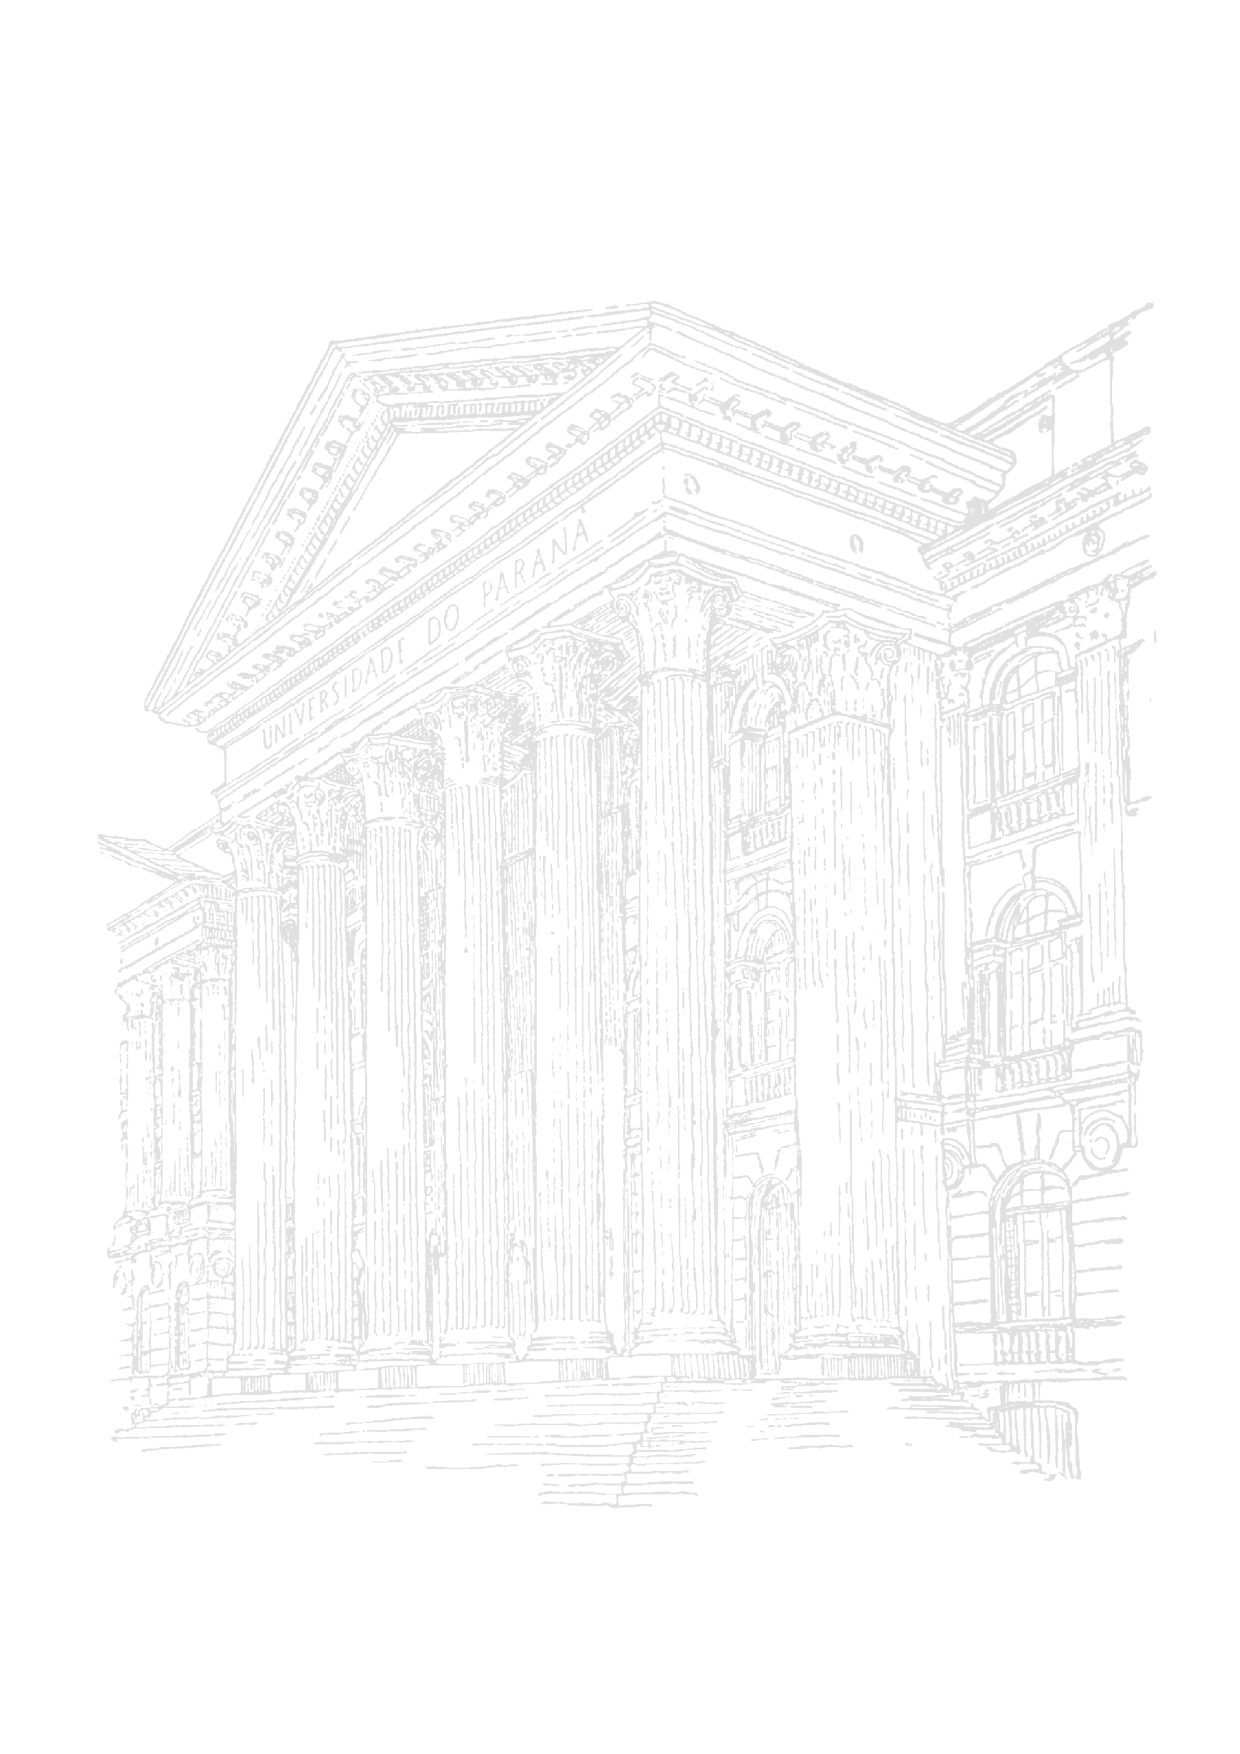
\includegraphics[width=\paperwidth,
  height=\paperheight]{images/ufpr_bg}};

\begin{center}
  {\Large \textsf{Universidade Federal do Paraná}}
  \vspace{-0.5cm}
\end{center}

\imprimircapa

% ---

% ---
% Folha de rosto
% ---
\imprimirfolhaderosto
% ---

% ---
% Dedicatória
% ---
% \begin{dedicatoria}
%   \lipsum[1]
% \end{dedicatoria}
% ---

% ---
% Agradecimentos
% ---
% \begin{agradecimentos}
%   \lipsum[1]
% \end{agradecimentos}
% ---

% ---
% Epígrafe
% ---
%\begin{epigrafe}
%    \vspace*{\fill}
%	\begin{flushright}
%          \textit{``Software is like sex: it's better when \\
%            it's free``}\\
%          --- Linus Torvalds \\[1cm]

%          \textit{``The numbers are where the scientific \\ discussion
%            should start, not end.''}\\
%          --- Steven N. Goodman
%	\end{flushright}
%\end{epigrafe}
% ---

% ---
% RESUMOS
% ---

% resumo em português
%\setlength{\absparsep}{18pt} % ajusta o espaçamento dos parágrafos do resumo
%\begin{resumo}


% ---
% inserir lista de ilustrações
% ---
%\pdfbookmark[0]{\listfigurename}{lof}
%\listoffigures*
%\cleardoublepage
% ---

% ---
% inserir lista de tabelas
% ---
%\pdfbookmark[0]{\listtablename}{lot}
%\listoftables*
%\cleardoublepage
% ---

% ---
% inserir lista de quadros
% ---
%\pdfbookmark[0]{\listofquadrosname}{loq}
%\listofquadros*
%\cleardoublepage
% ---

% ---
% inserir lista de abreviaturas e siglas
% ---
% \begin{siglas}
%   \item[ABNT] Associação Brasileira de Normas Técnicas
%   \item[abnTeX] ABsurdas Normas para TeX
% \end{siglas}
% ---

% ---
% inserir lista de símbolos
% ---
% \begin{simbolos}
%   \item[$ \log $] Logarítmo neperiano (de base $e$).
%   \item[$ \ell $] log-verossimilhança maximizada.
%   \item[AIC] Critério de Informação de Akaike, do inglês \textit{Akaike
%       Information Criterion}.
% \end{simbolos}
% ---

% ---
% inserir o sumario
% ---
\pdfbookmark[0]{\contentsname}{toc}
\tableofcontents*
\cleardoublepage
% ---

% ----------------------------------------------------------
% ELEMENTOS TEXTUAIS
% ----------------------------------------------------------
\textual

\chapter{Introdução}
\label{cap:introducao}

% ----------------------------------------------------------------------
% CAPÍTULO 1INTRODUÇÃO
% ----------------------------------------------------------------------

Aprendizado de máquina consiste em programar computadores de forma que eles aprendam a partir de dados. No cenário em que temos dados rotulados e uma variável alvo definida por categorias, recomenda-se o uso de técnicas de aprendizado supervisionado para fins de classificação. Dentre os diversos classificadores bem definidos e implementados, podemos citar o kNN, o Naive Bayes, a LDA, a regressão logística e o Perceptron.

A ideia geral do kNN consiste em, para uma unidade, encontrar os k mais próximos (similares) a ele e atribuir a classe mais frequente. Como existe a necessidade de obter a distância de um ponto para os outros, há um alto custo computacional. Outra característica deste classificador é que não requer treinamento, apenas teste, pois necessita apenas de distâncias. Contudo, a fase de teste demanda tempo considerável.

O Naive Bayes é um classificador baseado em probabilidade, mais especificamente, no pensamento bayesiano. Tem como base o teorema de Bayes, que consiste em alterar as probabilidades a priori (vindas dos vetores de característica) em estimativas de probabilidade a posteriori. A ideia do teorema é a revisão de crenças conforme surgem novas evidências e, na prática, atualiza-se a probabilidade a posteriori através da priori e da verossimilhança. O algoritmo, por sua vez, é chamado de ingênuo pois faz uma forte suposição: de que os atributos são independentes, contudo costuma apresentar bons resultados. O treinamento do Naive Bayes consiste na obtenção das probabilidades condicionais. Isto é, probabilidade da característica dado o desfecho. No caso de variáveis discretas, as probabilidades são beaseadas em frequências. Para contínuas as probabilidades comumente utilizadas são discretizar a variável em categorias ou usar uma função densidade de probabilidade (em geral, usa-se distribuição normal).

A LDA é um classificador baseado em transformações que tentam maximizar a distância entre classes e minimizar a distância intra classe. Na prática, o algoritmo busca encontrar a melhor projeção no espaço que discrimine as categorias. Trata-se de um classificador bastante simples e rápido, muito conhecido em contextos de redução de dimensionalidade. Além disso, é um modelo que apresenta certos pressupostos que, quando atendidos, geram resultados similares ao Naive Bayes, contudo, sem os pressupostos, ainda assim os resultados costumam ser satisfatórios.

A regressão logística é um classificador originalmente binário que apresenta uma característica bastante interessante: para fins de predição, fornece, além da classe, a probabilidade associada. Ou seja, a fronteira de decisão é baseada em um limiar de probabilidade. Além disso, apesar de se tratar de um classificador binário, diversas implementações adaptam este algoritmo para lidar com múltiplas classes. Trata-se de um método bastante atrativo principalmente porque costuma apresentar bons resultados em problemas desbalanceados.

O Perceptron é um classificador linear baseado numa rede neural de um único neurônio que funciona bem para problemas linearmente separáveis. Seu funcionamento se dá a partir de um vetor de entrada, que é associado a pesos. Esta informação é sumarizada, passada por uma função de ativação e o resultado final é a resposta. Os pesos são obtidos na fase de aprendizagem e trata-se de um algoritmo "online", isto é, a cada exemplo visto, os pesos são atualizados, o que gera um ajuste mais fino. Contudo, como a cada exemplo o modelo é revisto, os dados devem estar bem embaralhados para evitar o chamado \emph{Cathastrophic Forgetting} (convergir para uma única classe). Outra característica interessante do Perceptron é que, se o problema for linearmente separável, o algoritmo vai convergir e encontrar uma fronteira.

O objetivo deste relatório é apresentar os resultados da comparação de desempenho dos classificadores mencionados em função da disponibilidade da base de treinamento.


\chapter{Descrição da atividade}
\label{cap:descricao}

% ----------------------------------------------------------------------
% CAPÍTULO 2 - DESCRIÇÃO DAS ATIVIDADES
% ----------------------------------------------------------------------


O objetivo da tarefa é, considerando os classifcadores kNN, Naive Bayes, LDA, regressão logística e Perceptron, avaliar qual deles necessita de menos exemplos para aprender, qual tamanho de base de treinamento é suficiente para cada classificador, qual deles apresenta um melhor desempenho com poucos ou muitos dados, qual deles se mostra o mais rápido e ainda avaliar quais classificadores são complementares no problema sugerido.

Para o trabalho foram disponibilizados dois conjuntos de dados: um de treino e um de teste. Ambos os conjuntos referentes a um problema de classificação com 10 classes balanceadas e 132 características. A base de treino continha 20 mil exemplos e a de teste continha 58646.

Foi realizado um experimento no qual, para cada algoritmo, foram treinados 20 modelos aumentando o tamanho da base de treino de mil em mil, isto é, a primeira versão utilizava apenas 1000 exemplos para treinar, a segunda utilizava 2000 e assim por diante, até o último teste que utilizava todas as 20 mil observações no treinamento. Cada um destes modelos foi devidamente avaliado na base de teste, mantida fixa com todas as 58646 observações. Com isso, os resultados contém a análise de 20 modelos e 5 algoritmos, totalizando 100 cenários. Para cada cenário a métrica utilizada para avaliação foi a acurácia, considerando que trata-se de um problema balanceado.

Através da análise gráfica do comportamento da acurácia para cada classificador associado a cada tamanho de base de treinamento, buscou-se responder as perguntas inicialmente propostas. Após esta análise gráfica, explorou-se a matriz de confusão dos modelos que fizeram uso de toda a base de treinamento. 

Os modelos foram ajustados utilizando a biblioteca \emph{scikit-learn}, disponível para linguagem Python. Para execução do trabalho utilizou-se a plataforma Google Colaboratory (ou "Colab") que permite escrever código Python diretamente no navegador. Já a análise dos resultados foram realizadas no software R.

Quanto as parametrizações utilizadas para cada classificador no \emph{scikit-learn}: para os classificadores Naive Bayes, LDA e Perceptron foram utilizados os parâmetros default das funções \emph{GaussianNB()}, \emph{LinearDiscriminantAnalysis()} e \emph{Perceptron()}, respectivamente. Para o kNN, através da função \emph{KNeighborsClassifier()} foram utilizados 5 vizinhos, função peso uniforme, algoritmo kd\_tree, leaf\_size igual a 30, e distância de Minkowski com p igual a 2 (distância Euclideana). Para regressão logística, foi utilizada a função \emph{LogisticRegression()} utilizando algoritmo sag para otimização, indicado para problemas com conjuntos de dados grandes e número de iterações máximo igual a 500.

\chapter{Resultados obtidos}
\label{cap:resultados}

% ----------------------------------------------------------------------
% CAPÍTULO 3 - RESULTADOS OBTIDOS
% ----------------------------------------------------------------------

As representações gráficas dos resultados dos experimentos estão representadas nas Figuras 1 e 2. Em ambas, no eixo horizontal está representado o número de exemplos utilizados da base de treinamento. No eixo vertical é mostrada a acurácia. As cores representam cada classificador. Na Figura 1 é possível comparar melhor o desempenho de cada classificador de acordo com o tamanho da base de treino. A Figura 2, por sua vez, fornece uma visão mais clara de quais algoritmos apresentam comportamento mais estável e também daqueles mais instáveis.

Os resultados mostram que, considerando o cenário com o menor número de exemplos tomados para treinamento, a acurácia mais alta foi observada para LDA e kNN, fornecendo indicativo de que, em cenários com poucos dados disponíveis para treinamento, estas são boas escolhas. A pior acurácia no cenário com poucos dados foi observada para o Naive Bayes. Contudo, apesar de um resultado abaixo dos demais, notou-se que o Naive Bayes apresenta um considerável salto de acurácia nos três primeiros pontos (mil, 2 mil e 3 mil exemplos). 

A análise mostra ainda uma estabilidade na acurácia em todos os algoritmos a partir de 9 mil exemplos fornecidos para treino, isto é, o tamanho da base de treinamento deixa de ser relevante a partir de 9 mil. Avaliando a Figura 1, nota-se que, de 9 mil em diante, há um desempenho superior do kNN, seguido pela LDA, regressão logística e Naive Bayes. Estes quatro classificadores apresentam um padrão consideravelmente estável conforme aumenta-se o tamanho do treino. O Perceptron apresentou resultados satisfatórios em termos de acurácia, porém, comparado aos demais, apresentou grande oscilação. 

No cenário considerando toda a base de aprendizagem, Perceptron e kNN aparecem praticamente empatados. O Perceptron, apesar da já mencionada oscilação, parece apresentar uma tendência crescente de acurácia conforme aumenta-se o treino. Já o kNN apresenta aparente estabilidade desde muito cedo. Tais resultados são indicativos de que talvez o Perceptron poderia se mostrar superior aos demais com mais exemplos para treinamento.

A Figura 2 fornece uma visão mais geral da velocidade com que os classificadores se estabilizam. É possível notar que o Naive Bayes não chega em nenhum cenário a uma acurácia superior a 0.9, contudo existe um salto considerável na acurácia para poucos exemplos. O kNN apresentou boa escalabilidade de acurácia e uma grande estabilidade após determinado número de exemplos no treino. O LDA apresentou comportamento bastante similar ao kNN. A regressão logística apresentou uma curva mais lenta até a estabilizição da acurácia. Por fim, na Figura 2 fica ainda mais evidente as oscilações presentes no Perceptron.

Considerando os classificadores que usaram toda a base de treinamento, buscou-se avaliar quais eram complementares com o objetivo de conjecturar quais deles poderiam ser combinados para se obter um melhor resultado. Tal análise foi feita baseada na avaliação das matrizes de confusão para cada modelo, resultados apresentados nas Tabelas 1 e 2. 

Os resultados mostram que as classificações mais precisas na base de teste para as classes 0, 1, 3, 5 e 7 foram feitas pelo Perceptron. Já as classes 2, 6 e 8 foram melhores classificadas pelo kNN. A categoria 4 teve maior número de acertos quando utilizou-se regressão logística. Já para a categoria 9, LDA apresentou melhores resultados. Com isso, há indício de que os classificadores complementares são o kNN e o Perceptron.

\begin{table}[h]
\centering
\begin{tabular}{rcccccccccc}
\hline
\multicolumn{1}{r|}{\textbf{kNN}}         & \textbf{0}                         & \textbf{1}                         & \textbf{2}                         & \textbf{3}                         & \textbf{4}                         & \textbf{5}                         & \textbf{6}                         & \textbf{7}                         & \textbf{8}                         & \textbf{9}                         \\ \hline
\multicolumn{1}{r|}{\textbf{0}}           & \multicolumn{1}{c|}{\textbf{5472}} & 3                                  & 1                                  & 15                                 & 6                                  & 2                                  & 26                                 & 2                                  & 32                                 & 1                                  \\ \cline{2-3}
\multicolumn{1}{r|}{\textbf{1}}           & \multicolumn{1}{c|}{0}             & \multicolumn{1}{c|}{\textbf{6105}} & 175                                & 119                                & 56                                 & 6                                  & 35                                 & 66                                 & 34                                 & 59                                 \\ \cline{3-4}
\multicolumn{1}{r|}{\textbf{2}}           & 12                                 & \multicolumn{1}{c|}{11}            & \multicolumn{1}{c|}{\textbf{5607}} & 165                                & 3                                  & 1                                  & 16                                 & 51                                 & 20                                 & 2                                  \\ \cline{4-5}
\multicolumn{1}{r|}{\textbf{3}}           & 4                                  & 1                                  & \multicolumn{1}{c|}{25}            & \multicolumn{1}{c|}{\textbf{5646}} & 2                                  & 51                                 & 1                                  & 53                                 & 20                                 & 16                                 \\ \cline{5-6}
\multicolumn{1}{r|}{\textbf{4}}           & 12                                 & 11                                 & 13                                 & \multicolumn{1}{c|}{3}             & \multicolumn{1}{c|}{\textbf{5305}} & 9                                  & 132                                & 24                                 & 11                                 & 202                                \\ \cline{6-7}
\multicolumn{1}{r|}{\textbf{5}}           & 9                                  & 3                                  & 9                                  & 489                                & \multicolumn{1}{c|}{4}             & \multicolumn{1}{c|}{\textbf{4842}} & 41                                 & 16                                 & 83                                 & 43                                 \\ \cline{7-8}
\multicolumn{1}{r|}{\textbf{6}}           & 31                                 & 10                                 & 4                                  & 2                                  & 3                                  & \multicolumn{1}{c|}{44}            & \multicolumn{1}{c|}{\textbf{5724}} & 0                                  & 40                                 & 0                                  \\ \cline{8-9}
\multicolumn{1}{r|}{\textbf{7}}           & 1                                  & 25                                 & 41                                 & 119                                & 54                                 & 1                                  & \multicolumn{1}{c|}{0}             & \multicolumn{1}{c|}{\textbf{5773}} & 7                                  & 76                                 \\ \cline{9-10}
\multicolumn{1}{r|}{\textbf{8}}           & 36                                 & 24                                 & 42                                 & 114                                & 32                                 & 38                                 & 50                                 & \multicolumn{1}{c|}{27}            & \multicolumn{1}{c|}{\textbf{5165}} & 167                                \\ \cline{10-11} 
\multicolumn{1}{r|}{\textbf{9}}           & 16                                 & 9                                  & 17                                 & 107                                & 78                                 & 9                                  & 9                                  & 131                                & \multicolumn{1}{c|}{34}            & \multicolumn{1}{c|}{\textbf{5403}} \\ \hline
\textbf{}                                 &                                    &                                    &                                    &                                    &                                    &                                    &                                    &                                    &                                    &                                    \\ \hline
\multicolumn{1}{c|}{\textbf{Naive Bayes}} & \textbf{0}                         & \textbf{1}                         & \textbf{2}                         & \textbf{3}                         & \textbf{4}                         & \textbf{5}                         & \textbf{6}                         & \textbf{7}                         & \textbf{8}                         & \textbf{9}                         \\ \hline
\multicolumn{1}{r|}{\textbf{0}}           & \multicolumn{1}{c|}{\textbf{5220}} & 1                                  & 11                                 & 32                                 & 2                                  & 1                                  & 41                                 & 0                                  & 251                                & 1                                  \\ \cline{2-3}
\multicolumn{1}{r|}{\textbf{1}}           & \multicolumn{1}{c|}{1}             & \multicolumn{1}{c|}{\textbf{5184}} & 583                                & 238                                & 86                                 & 22                                 & 85                                 & 340                                & 80                                 & 36                                 \\ \cline{3-4}
\multicolumn{1}{r|}{\textbf{2}}           & 9                                  & \multicolumn{1}{c|}{24}            & \multicolumn{1}{c|}{\textbf{5289}} & 447                                & 4                                  & 1                                  & 8                                  & 52                                 & 53                                 & 1                                  \\ \cline{4-5}
\multicolumn{1}{r|}{\textbf{3}}           & 2                                  & 1                                  & \multicolumn{1}{c|}{212}           & \multicolumn{1}{c|}{\textbf{5390}} & 1                                  & 33                                 & 0                                  & 127                                & 31                                 & 22                                 \\ \cline{5-6}
\multicolumn{1}{r|}{\textbf{4}}           & 14                                 & 2                                  & 44                                 & \multicolumn{1}{c|}{12}            & \multicolumn{1}{c|}{\textbf{5273}} & 0                                  & 32                                 & 44                                 & 90                                 & 211                                \\ \cline{6-7}
\multicolumn{1}{r|}{\textbf{5}}           & 9                                  & 6                                  & 29                                 & 103                                & \multicolumn{1}{c|}{31}            & \multicolumn{1}{c|}{\textbf{4958}} & 46                                 & 2                                  & 169                                & 186                                \\ \cline{7-8}
\multicolumn{1}{r|}{\textbf{6}}           & 78                                 & 7                                  & 89                                 & 8                                  & 15                                 & \multicolumn{1}{c|}{90}            & \multicolumn{1}{c|}{\textbf{5286}} & 0                                  & 285                                & 0                                  \\ \cline{8-9}
\multicolumn{1}{r|}{\textbf{7}}           & 1                                  & 47                                 & 175                                & 426                                & 21                                 & 1                                  & \multicolumn{1}{c|}{1}             & \multicolumn{1}{c|}{\textbf{5323}} & 60                                 & 42                                 \\ \cline{9-10}
\multicolumn{1}{r|}{\textbf{8}}           & 175                                & 5                                  & 53                                 & 182                                & 23                                 & 7                                  & 38                                 & \multicolumn{1}{c|}{13}            & \multicolumn{1}{c|}{\textbf{5112}} & 87                                 \\ \cline{10-11} 
\multicolumn{1}{r|}{\textbf{9}}           & 25                                 & 5                                  & 62                                 & 151                                & 221                                & 4                                  & 0                                  & 55                                 & \multicolumn{1}{c|}{184}           & \multicolumn{1}{c|}{\textbf{5106}} \\ \hline
\textbf{}                                 &                                    &                                    &                                    &                                    &                                    &                                    &                                    &                                    &                                    &                                   
\end{tabular}
\caption{Matrizes de confusão kNN e Naive Bayes.}
\label{tab:cm1}
\end{table}

\begin{table}[h]
\centering
\begin{tabular}{rcccccccccc}
\hline
\multicolumn{1}{r|}{\textbf{LDA}}        & \textbf{0}                         & \textbf{1}                         & \textbf{2}                         & \textbf{3}                         & \textbf{4}                         & \textbf{5}                         & \textbf{6}                         & \textbf{7}                         & \textbf{8}                         & \textbf{9}                         \\ \hline
\multicolumn{1}{r|}{\textbf{0}}          & \multicolumn{1}{c|}{\textbf{5358}} & 10                                 & 11                                 & 15                                 & 19                                 & 0                                  & 47                                 & 17                                 & 80                                 & 3                                  \\ \cline{2-3}
\multicolumn{1}{r|}{\textbf{1}}          & \multicolumn{1}{c|}{0}             & \multicolumn{1}{c|}{\textbf{6027}} & 222                                & 85                                 & 9                                  & 22                                 & 38                                 & 199                                & 31                                 & 22                                 \\ \cline{3-4}
\multicolumn{1}{r|}{\textbf{2}}          & 22                                 & \multicolumn{1}{c|}{41}            & \multicolumn{1}{c|}{\textbf{5605}} & 12                                 & 1                                  & 0                                  & 4                                  & 175                                & 27                                 & 1                                  \\ \cline{4-5}
\multicolumn{1}{r|}{\textbf{3}}          & 1                                  & 12                                 & \multicolumn{1}{c|}{29}            & \multicolumn{1}{c|}{\textbf{5470}} & 1                                  & 19                                 & 1                                  & 247                                & 23                                 & 16                                 \\ \cline{5-6}
\multicolumn{1}{r|}{\textbf{4}}          & 20                                 & 71                                 & 42                                 & \multicolumn{1}{c|}{0}             & \multicolumn{1}{c|}{\textbf{5208}} & 0                                  & 86                                 & 5                                  & 29                                 & 261                                \\ \cline{6-7}
\multicolumn{1}{r|}{\textbf{5}}          & 9                                  & 11                                 & 6                                  & 314                                & \multicolumn{1}{c|}{4}             & \multicolumn{1}{c|}{\textbf{5015}} & 50                                 & 24                                 & 67                                 & 39                                 \\ \cline{7-8}
\multicolumn{1}{r|}{\textbf{6}}          & 77                                 & 49                                 & 37                                 & 15                                 & 56                                 & \multicolumn{1}{c|}{36}            & \multicolumn{1}{c|}{\textbf{5460}} & 0                                  & 125                                & 3                                  \\ \cline{8-9}
\multicolumn{1}{r|}{\textbf{7}}          & 0                                  & 58                                 & 47                                 & 6                                  & 58                                 & 1                                  & \multicolumn{1}{c|}{0}             & \multicolumn{1}{c|}{\textbf{5882}} & 22                                 & 23                                 \\ \cline{9-10}
\multicolumn{1}{r|}{\textbf{8}}          & 80                                 & 59                                 & 38                                 & 5                                  & 51                                 & 29                                 & 54                                 & \multicolumn{1}{c|}{57}            & \multicolumn{1}{c|}{\textbf{4961}} & 361                                \\ \cline{10-11} 
\multicolumn{1}{r|}{\textbf{9}}          & 34                                 & 31                                 & 9                                  & 91                                 & 69                                 & 7                                  & 16                                 & 98                                 & \multicolumn{1}{c|}{29}            & \multicolumn{1}{c|}{\textbf{5429}} \\ \hline
\textbf{}                                &                                    &                                    &                                    &                                    &                                    &                                    &                                    &                                    &                                    &                                    \\ \hline
\multicolumn{1}{r|}{\textbf{Reg. Log.}}  & \textbf{0}                         & \textbf{1}                         & \textbf{2}                         & \textbf{3}                         & \textbf{4}                         & \textbf{5}                         & \textbf{6}                         & \textbf{7}                         & \textbf{8}                         & \textbf{9}                         \\ \hline
\multicolumn{1}{r|}{\textbf{0}}          & \multicolumn{1}{c|}{\textbf{5381}} & 5                                  & 16                                 & 12                                 & 15                                 & 4                                  & 69                                 & 6                                  & 51                                 & 1                                  \\ \cline{2-3}
\multicolumn{1}{r|}{\textbf{1}}          & \multicolumn{1}{c|}{1}             & \multicolumn{1}{c|}{\textbf{5595}} & 116                                & 269                                & 200                                & 74                                 & 179                                & 74                                 & 78                                 & 69                                 \\ \cline{3-4}
\multicolumn{1}{r|}{\textbf{2}}          & 22                                 & \multicolumn{1}{c|}{18}            & \multicolumn{1}{c|}{\textbf{5585}} & 89                                 & 12                                 & 1                                  & 33                                 & 82                                 & 45                                 & 1                                  \\ \cline{4-5}
\multicolumn{1}{r|}{\textbf{3}}          & 4                                  & 3                                  & \multicolumn{1}{c|}{37}            & \multicolumn{1}{c|}{\textbf{5597}} & 16                                 & 39                                 & 1                                  & 74                                 & 20                                 & 28                                 \\ \cline{5-6}
\multicolumn{1}{r|}{\textbf{4}}          & 35                                 & 8                                  & 30                                 & \multicolumn{1}{c|}{1}             & \multicolumn{1}{c|}{\textbf{5315}} & 2                                  & 104                                & 41                                 & 9                                  & 177                                \\ \cline{6-7}
\multicolumn{1}{r|}{\textbf{5}}          & 6                                  & 12                                 & 23                                 & 497                                & \multicolumn{1}{c|}{78}            & \multicolumn{1}{c|}{\textbf{4728}} & 50                                 & 22                                 & 73                                 & 50                                 \\ \cline{7-8}
\multicolumn{1}{r|}{\textbf{6}}          & 87                                 & 26                                 & 0                                  & 1                                  & 20                                 & \multicolumn{1}{c|}{96}            & \multicolumn{1}{c|}{\textbf{5517}} & 0                                  & 111                                & 0                                  \\ \cline{8-9}
\multicolumn{1}{r|}{\textbf{7}}          & 0                                  & 41                                 & 40                                 & 121                                & 165                                & 2                                  & \multicolumn{1}{c|}{0}             & \multicolumn{1}{c|}{\textbf{5600}} & 17                                 & 111                                \\ \cline{9-10}
\multicolumn{1}{r|}{\textbf{8}}          & 83                                 & 43                                 & 47                                 & 59                                 & 85                                 & 46                                 & 53                                 & \multicolumn{1}{c|}{58}            & \multicolumn{1}{c|}{\textbf{5000}} & 221                                \\ \cline{10-11} 
\multicolumn{1}{r|}{\textbf{9}}          & 55                                 & 22                                 & 8                                  & 143                                & 251                                & 0                                  & 4                                  & 150                                & \multicolumn{1}{c|}{19}            & \multicolumn{1}{c|}{\textbf{5161}} \\ \hline
\textbf{}                                &                                    &                                    &                                    &                                    &                                    &                                    &                                    &                                    &                                    &                                    \\ \hline
\multicolumn{1}{r|}{\textbf{Perceptron}} & \textbf{0}                         & \textbf{1}                         & \textbf{2}                         & \textbf{3}                         & \textbf{4}                         & \textbf{5}                         & \textbf{6}                         & \textbf{7}                         & \textbf{8}                         & \textbf{9}                         \\ \hline
\multicolumn{1}{r|}{\textbf{0}}          & \multicolumn{1}{c|}{\textbf{5532}} & 1                                  & 0                                  & 6                                  & 0                                  & 1                                  & 18                                 & 1                                  & 1                                  & 0                                  \\ \cline{2-3}
\multicolumn{1}{r|}{\textbf{1}}          & \multicolumn{1}{c|}{14}            & \multicolumn{1}{c|}{\textbf{6114}} & 46                                 & 217                                & 14                                 & 176                                & 27                                 & 43                                 & 2                                  & 2                                  \\ \cline{3-4}
\multicolumn{1}{r|}{\textbf{2}}          & 88                                 & \multicolumn{1}{c|}{32}            & \multicolumn{1}{c|}{\textbf{5548}} & 137                                & 2                                  & 0                                  & 16                                 & 62                                 & 3                                  & 0                                  \\ \cline{4-5}
\multicolumn{1}{r|}{\textbf{3}}          & 5                                  & 3                                  & \multicolumn{1}{c|}{12}            & \multicolumn{1}{c|}{\textbf{5698}} & 0                                  & 60                                 & 1                                  & 28                                 & 2                                  & 10                                 \\ \cline{5-6}
\multicolumn{1}{r|}{\textbf{4}}          & 116                                & 13                                 & 46                                 & \multicolumn{1}{c|}{17}            & \multicolumn{1}{c|}{\textbf{5172}} & 7                                  & 108                                & 39                                 & 5                                  & 199                                \\ \cline{6-7}
\multicolumn{1}{r|}{\textbf{5}}          & 21                                 & 5                                  & 4                                  & 129                                & \multicolumn{1}{c|}{3}             & \multicolumn{1}{c|}{\textbf{5318}} & 40                                 & 1                                  & 6                                  & 12                                 \\ \cline{7-8}
\multicolumn{1}{r|}{\textbf{6}}          & 129                                & 8                                  & 5                                  & 4                                  & 5                                  & \multicolumn{1}{c|}{57}            & \multicolumn{1}{c|}{\textbf{5648}} & 0                                  & 2                                  & 0                                  \\ \cline{8-9}
\multicolumn{1}{r|}{\textbf{7}}          & 2                                  & 42                                 & 51                                 & 157                                & 31                                 & 4                                  & \multicolumn{1}{c|}{0}             & \multicolumn{1}{c|}{\textbf{5796}} & 1                                  & 13                                 \\ \cline{9-10}
\multicolumn{1}{r|}{\textbf{8}}          & 329                                & 39                                 & 45                                 & 457                                & 35                                 & 225                                & 185                                & \multicolumn{1}{c|}{20}            & \multicolumn{1}{c|}{\textbf{4211}} & 149                                \\ \cline{10-11} 
\multicolumn{1}{r|}{\textbf{9}}          & 89                                 & 36                                 & 26                                 & 115                                & 106                                & 25                                 & 3                                  & 83                                 & \multicolumn{1}{c|}{3}             & \multicolumn{1}{c|}{\textbf{5327}} \\ \hline
\end{tabular}
\caption{Matrizes de confusão LDA, regressão logística e Perceptron.}
\label{tab:cm2}
\end{table}

\begin{landscape}

\begin{figure}[]
\label{fig:fig1}
\centering
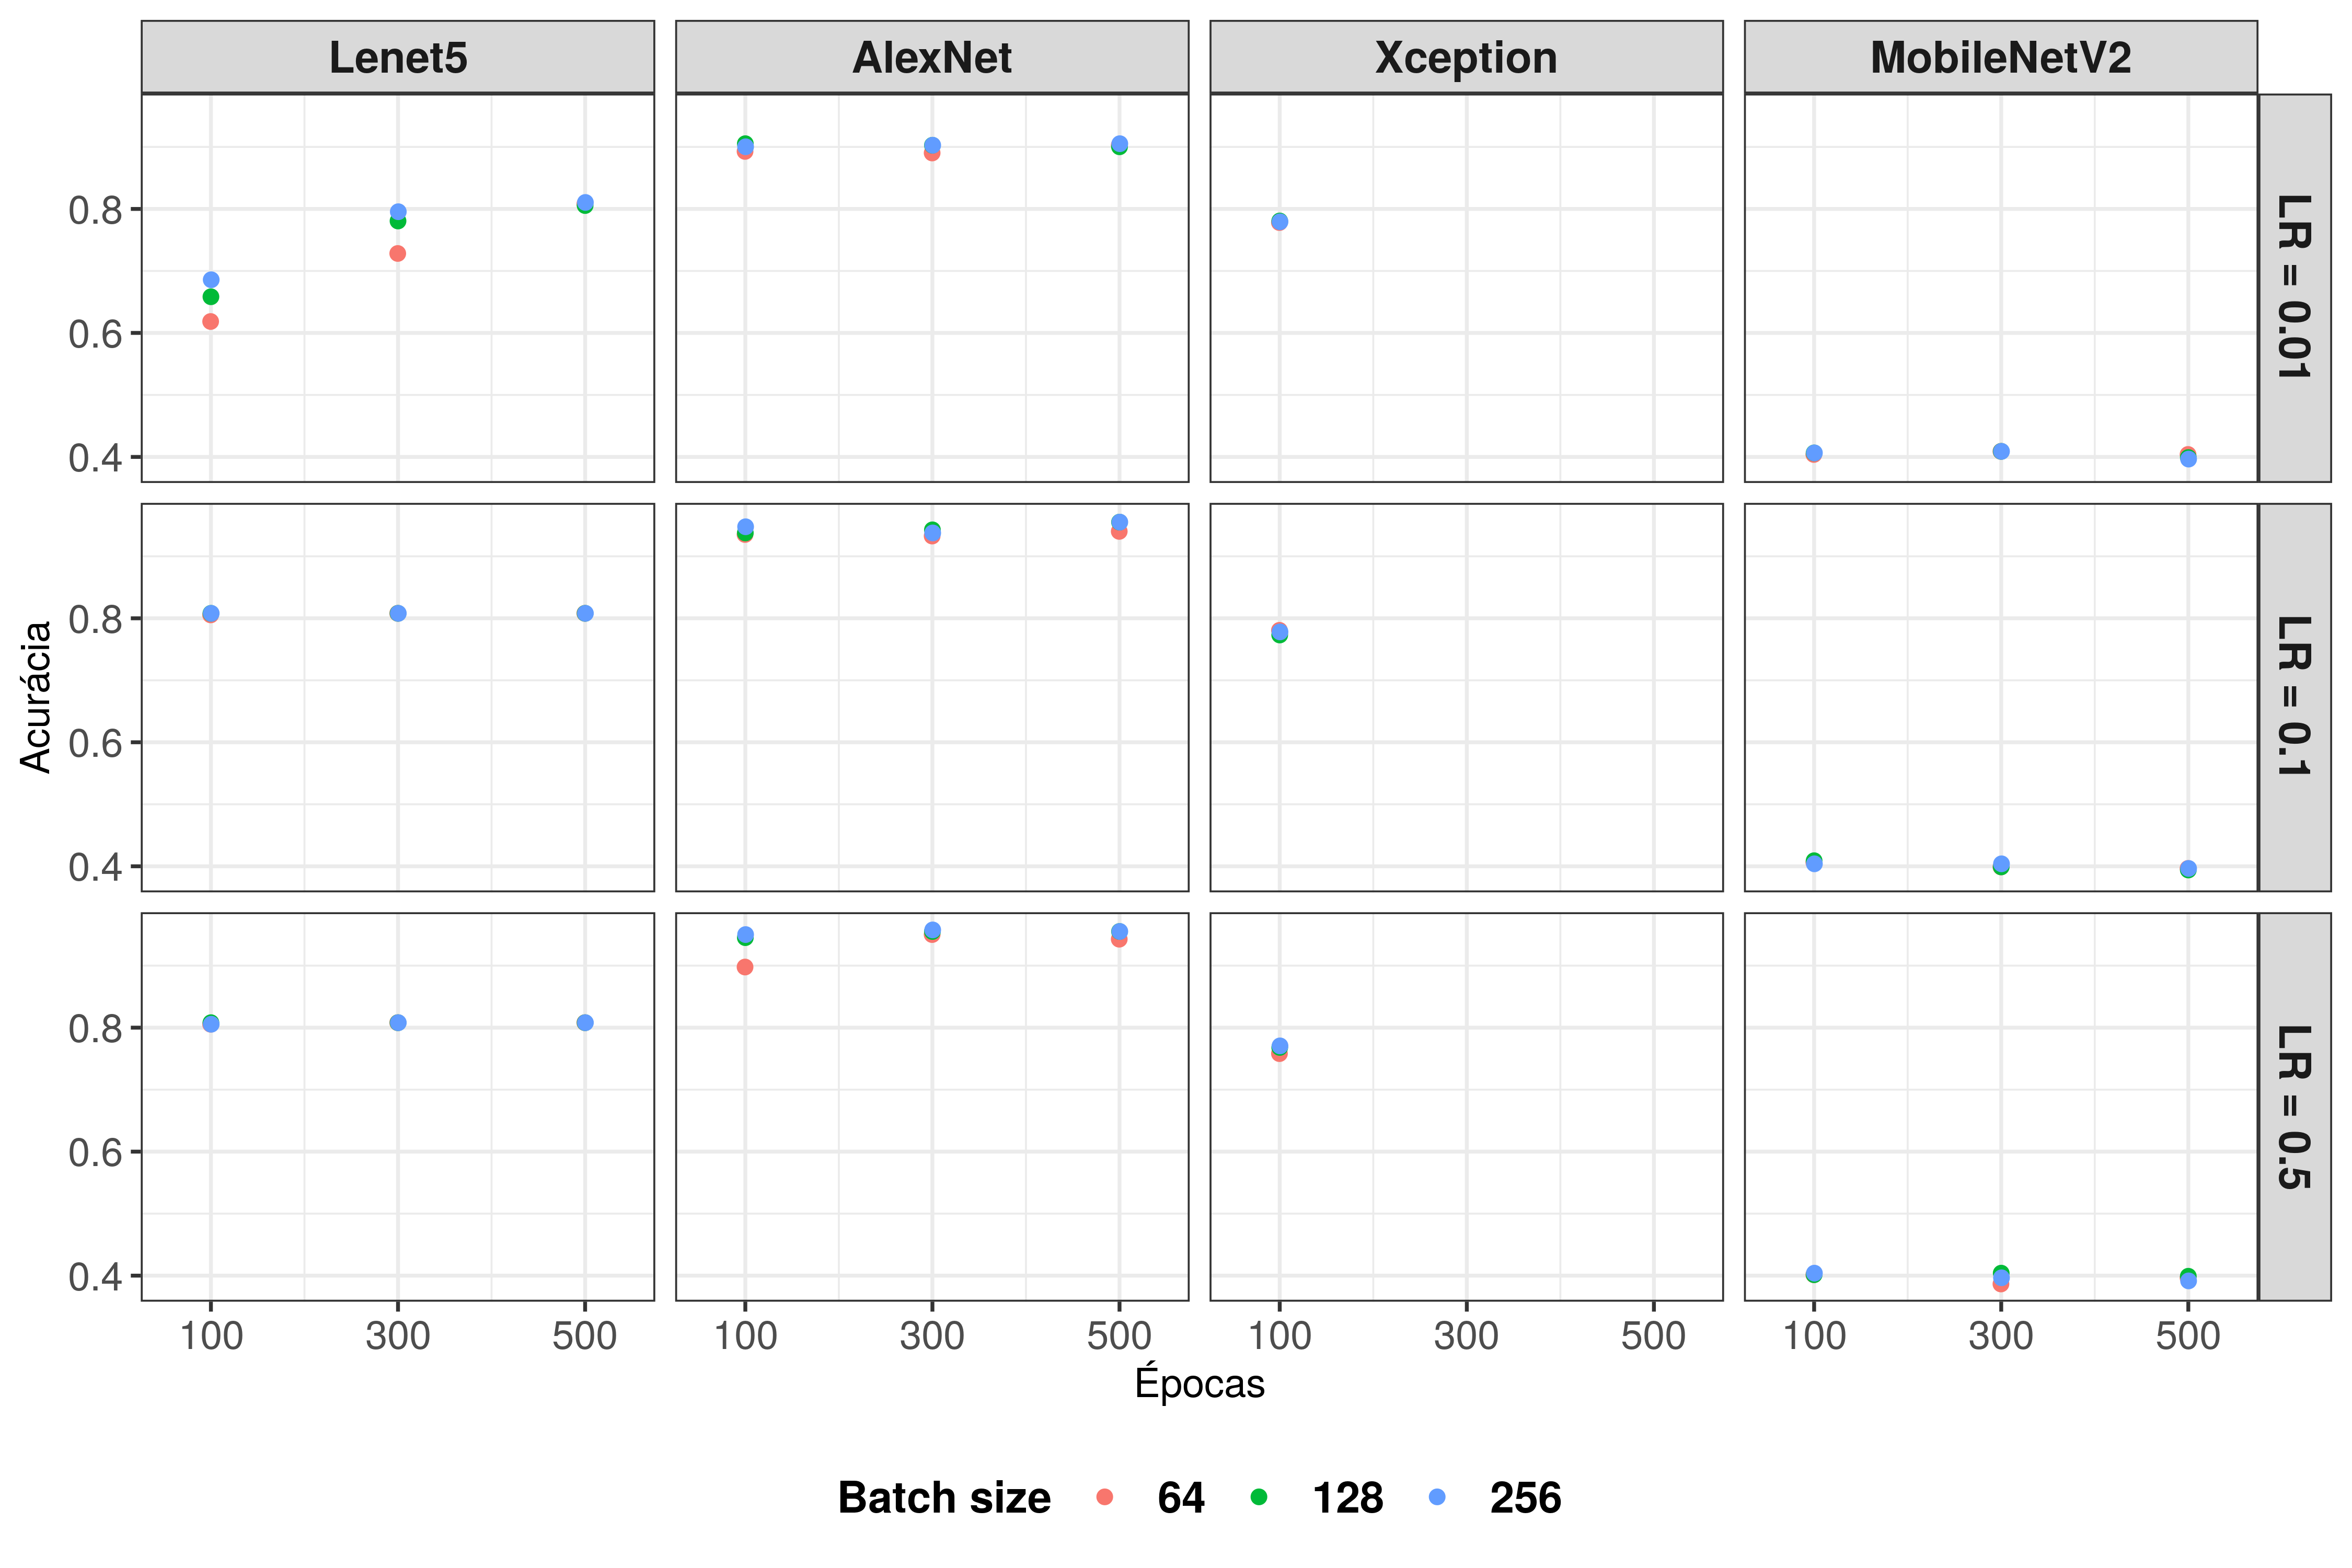
\includegraphics[width=1.6\textwidth]{/home/lacf14/machine_learning_ufpr/lab02/fig.png}
\caption{Acurácia na base de teste em função do número de exemplos usado no treino.}
\end{figure}
\end{landscape}

\begin{landscape}

\begin{figure}[]
\label{fig:fig2}
\centering
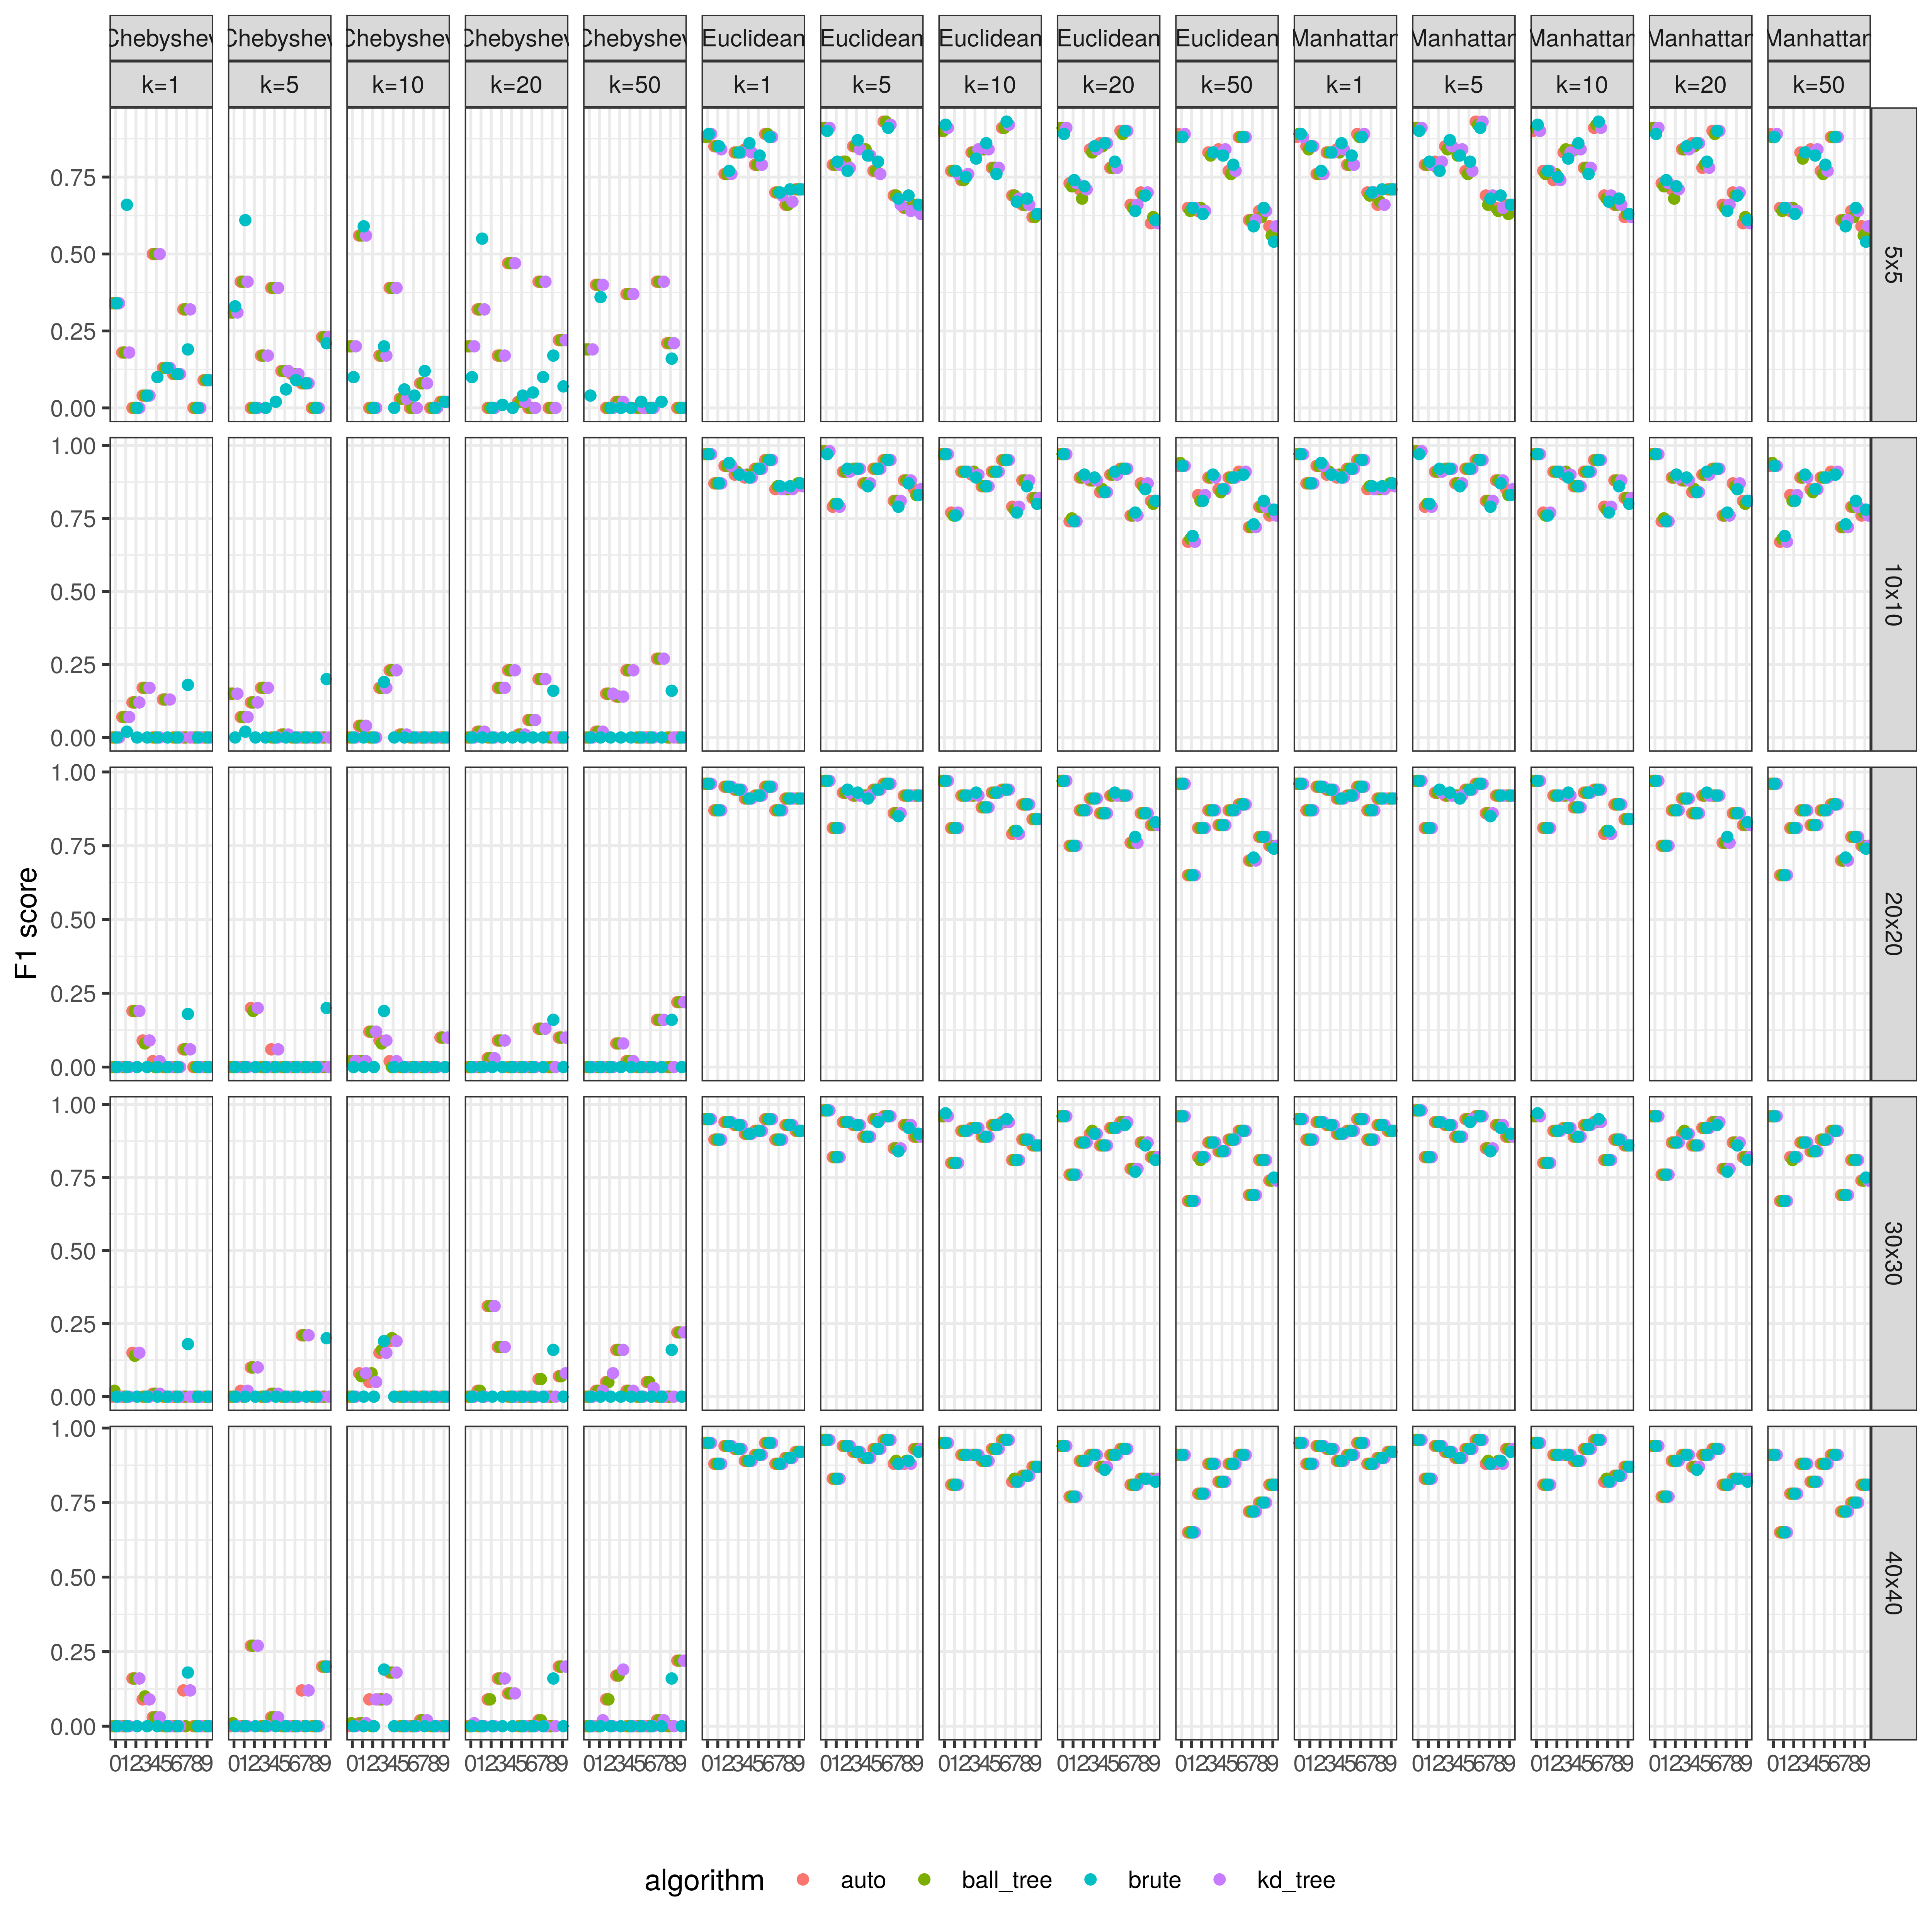
\includegraphics[width=1.6\textwidth]{/home/lacf14/machine_learning_ufpr/lab02/fig2.png}
\caption{Acurácia na base de teste em função do número de exemplos usado no treino (painel).}
\end{figure}
\end{landscape}

\chapter{Considerações finais}
\label{cap:conclusao}

% ----------------------------------------------------------------------
% CAPÍTULO 5 - CONCLUSÃO
% ----------------------------------------------------------------------

Os resultados mostraram que, neste problema, considerando poucos exemplos, a acurácia mais alta foi observada para LDA e kNN. Ou seja, este estudo sugere que com poucos dados disponíveis para treinamento estas escolhas são atrativas. O estudo sugere ainda que, para este problema, um lote de exemplos superior a 9 mil não traz grandes benefícios no treino dos algoritmos. Quanto a velocidade de classificação das 58646 unidades para teste, a única que se mostrou demorada foi o kNN, tomando aproximadamente 3 minutos na plataforma Google Colab. Os demais classificadores se mostraram bastante rápidos.

Quanto à acurácia dos classificadores testados verificou-se um desempenho superior do kNN, seguido pela LDA, regressão logística e Naive Bayes. O kNN apresentou boa escalabilidade de acurácia e uma grande estabilidade. Como esperado, o LDA apresentou comportamento bastante similar ao kNN, porém levemente inferior. Comparado aos demais, a regressão logística se mostrou sensível ao tamanho da base de treino, necessitando de uma base maior para atingir acurácia à altura dos demais. Notou-se também que, para bases pequenas de treinamento, regressão logística foi inferior ao Naive Bayes; contudo, para bases maiores, este padrão se inverte. O Perceptron apresentou grandes oscilações conforme alterava-se o tamanho da base, mas no cenário com toda a base de treinamento, se mostrou como o melhor classificador para o problema.

Considerando toda a base de aprendizagem, Perceptron e kNN apresentam acurácia bastante similar. Notou-se que o Perceptron oscilou consideravelmente, mas parece apresentar uma acurácia crescente e estabilizando, sugerindo que é um bom candidato para bases de treinamento mais volumosas. O kNN, por sua vez, se mostrou mais estável. Deste modo, uma escolha segura seria o kNN, uma escolha mais arriscada e que necessitaria de mais dados para treino seria o Perceptron. Além disso, estes classificadores se mostraram complementares, dando indídio de que uma combinação entre eles pode gerar um classificador mais poderoso para o problema em questão.

Por fim, vale ressaltar que esta análise foi meramente exploratória e para um estudo mais consistente o ideal seria trabalhar com replicação, isto é, em vez de selecionar lotes de mil da base fornecida, selecionar mil linhas ao acaso, obter os modelos, acurácia e repetir este procedimento algumas vezes para cada modelo. Deste modo seria possível obter estimativas pontuais e intervalares da acurácia para cada cenário, fornecendo uma ideia mais realista de quais deles são mais estáveis.

% ---
\phantompart

% ---
% Conclusão
% ---

% ----------------------------------------------------------
% ELEMENTOS PÓS-TEXTUAIS
% ----------------------------------------------------------
\postextual

% ----------------------------------------------------------
% Referências bibliográficas
% ----------------------------------------------------------

%% Utilize este na elaboração do documento
\bibliography{refs}

%% Utilize este apenas ao final, quando não forem mais realizadas
%% alterações
% \begin{flushleft}
%   \small
% \renewcommand\refname{}
% \vspace*{-1.5cm}
% \input{01-tcc_corrigido.bbl}
% \end{flushleft}

% ----------------------------------------------------------
% Apêndices
% ----------------------------------------------------------

% ---
% Inicia os apêndices
% ---
% \begin{apendicesenv}

% Imprime uma página indicando o início dos apêndices
% \partapendices

% \chapter{Programas R}
% \label{capA:codigostcc}

% \end{apendicesenv}
% ---

% ----------------------------------------------------------
% Anexos
% ----------------------------------------------------------

%% % ---
%% % Inicia os anexos
%% % ---
%% \begin{anexosenv}
%% % Imprime uma página indicando o início dos anexos
%% \partanexos
%% \chapter{Lipsum}
%% \lipsum[30]
%% \end{anexosenv}

%---------------------------------------------------------------------
% INDICE REMISSIVO
%---------------------------------------------------------------------
% \phantompart
% \printindex
%---------------------------------------------------------------------

\end{document}
